\section{Оптимизация параллельного обхода ограничений для GPU} \label{ch3:chunks}
	В рамках данной работы, перед автором стояла задача не только разработки эвристического алгоритма, описанного в параграфе \ref{ch3:heuristic}, но и реализации с использованием GPU. Действительно, главной отличительной особенностью GPU относительно CPU является много большее количество вычислительных ядер. Таким образом, учитывая закон Амдала, некоторые алгоритмы могут быть многократно ускорены за счет грамотного разбиения на подзадачи. Лучше всего GPU справляется в ситуации, когда вышеупомянутые подзадачи являются вычислительными задачами имеющими одинаковый алгоритм решения, однако разные входные данные. Подход, в котором GPU используется для вычисления задач общего назначения, не связанных с отображением графики, принято называть GPGPU - General-purpose computing on graphics processing units. Для реализации данного подхода есть два пути: либо использование специализированных библиотек для GPGPU, таких как Nvidia CUDA или OpenCL, либо использование вычислительных шейдеров в графических библиотеках, таких как DirectX12 или OpenGL. В рамках данной работы, автором рассматривается применение вычислительных шейдеров, так как конечной целью является встраивание симуляции тканей в приложение, использующее DirectX12.
	
	Введем некоторые основные понятия программирования в парадигме GPGPU. Если говорить с точки зрения выполнения, то на GPU запускаются шейдеры. Шейдеры запускаются параллельно, имеют одинаковый код, но получают различающийся входной аргумент - номер соответствующего потока исполнения. Потоки объединяются в группы, причем все группы имеет одинаковый размер. Программист же, при отправке команды на запуск какого-либо шейдера, указывает целое количество групп, которые он хочет выполнить. Для запуска каждой группы GPU выделяет целое число $Wavefront$-ов - наборов из процессоров, которые выполняют операции абсолютно параллельно. В случае использования видеокарт Nvidia размер одного $Wavefront$-а равен 32, а в случае AMD - 64.
	
	Если говорить с точки зрения памяти, каждый поток имеет локальную память (для локальных переменных шейдера), глобальную память (для считывания входных параметров и записи результирующих) и $groupshared$ память. Последняя является более быстрой по времени чтения-записи по отношению к глобальной, однако выделяется только в рамках запуска одной группы и может быть использована потоками внутри группы для обмена данными.
	
	Если же говорить с точки зрения синхронизации, то в рамках языка HLSL и DirectX12, есть два способа синхронизации вычислительных шейдеров:
	\begin{enumerate}[1.]
		\item Применение барьера глобальной памяти, в которую записывается результат. Таким образом, следующие команды не начнут выполняться до тех пор, пока каждая группа не закончит записывать в данную память.
		\item Использование команды шейдера $GroupMemoryBarrierWithGroupSync$, которая позволяет синхронизировать все $Wavefront$-ы внутри одной группы.
	\end{enumerate}
	
	Рассмотрим алгоритм XPBD, представленный на \firef{alg:HeuristicXPBD}, и перепишем его в виде, подходящем для параллельного выполнения (\firef{alg:HeuristicParallelXPBD}).

\begin{algorithm} [h]
	\SetKwFunction{algoXPBDParallelPseudocode}{} 
	\SetKwProg{myalg}{Algorithm}{}{} %write in 2nd agrument <<Algorithm>>, <<Procedure>> etc
	\nonl\myalg{\algoXPBDParallelPseudocode}{
		\For{$step \in 1..solverStep$}{			
			\If{$mod(step, HeuristicStep) = 0$}
			{
				\ForPar{$getHorRopes()$}
				{
					$ImprovedHeuristicAlgorithm()$
				}
				
				$syncPoint()$;
				
				\ForPar{$getVerRopes()$}
				{
					$ImprovedHeuristicAlgorithm()$
				}
			}
			
			\lForPar{$getParticles()$}
			{
				$predictParticle()$
			}
			
			$syncPoint()$;
			
			\lForPar{$getParticles()$}
			{
				$genCollisionConstraint()$
			}
			
			$syncPoint()$;
			
			\For{$type \in \{structural, shear, bending\}$}
			{
				\For{$color \in getColors(type)$}
				{
					\ForPar{$getConstraints(type, color)$}
					{
						$solveXPBDConstraint()$;
					}
					
					$syncPoint()$;
				}				
			}
			
			\ForPar{$getCollisionConstraints()$}
			{
				$solveCollisionConstaint()$;
			}
			
			$syncPoint()$;
						
			\lForPar{$getParticles()$}
			{
				$saveNewParticlePos()$
			}		
			
			$syncPoint()$;
		}
	}
	\caption{Псевдокод алгоритма Extended Position Based Dynamics с использованием Small steps, эвристического алгоритма и отмеченными местами возможной параллелизации}\label{alg:HeuristicParallelXPBD}
\end{algorithm}

	Как можно заметить, данный алгоритм отлично разбивается на подзадачи, имеющие одинаковый алгоритм, но разные входные данные, что прекрасно лосогласуется с использованием технологии GPGPU. Однако возникает вопрос: как именно реализовать данный алгоритм для выполнения при помощи GPU.
	
	Первый вариант: представить весь этот алгоритм как единый шейдер, для которого будет запущена только одна группа (такое решение используется в NVidia Cloth). Тогда каждый $syncPoint$ будет представлен как вызов $GroupMemoryBarrierWithGroupSync$, а частицы и ограничения сначала должны быть загружены в $groupshared$ память, а после окончания работы данного алгоритма выгружены обратно в глобальную. Недостатком данного подхода является то, что размер группы в языке HLSL не может превышать 1024, а значит невозможно использовать более 1024 потоков.
	
	Второй вариант: представить каждый \say{\textbf{for} * \textbf{do in parallel}} как отдельный шейдер. Тогда каждый $syncPoint$ будет представлен как выставление барьера. Недостатком данного подхода является то, что не используется $groupshared$ память, тем самым алгоритм теряет в производительности из-за многочисленных записей и чтений из глобальной памяти. Также, недостатком является частая смена и вызов различных шейдеров, что привносит дополнительные расходы по времени выполнения.
	
	В рамках исследования алгоритма XPBD с использованием техники Small steps и обходом ограничений на основании реберной раскраски было замечено, что в течение одной итерации вляние частиц ограничено. Это означает, что для подсчета положения конкретной частицы на следующей итерации необходимо знать положение лишь некоторых соседних частиц, а не всей ткани.
	
	Для определения границ влияния частиц был поставлен следующий эксперимент:
	\begin{enumerate}[1.]
		\item Строится сетка размером $(N+2)$ на $(N+2)$ вершины, соединенные между собой аналогично тому, как частицы ткани соединены структурными ограничениями
		\item Внешние вершины сетки отмечаются красным цветом, в то время как внутренние ограничения помечаются синим
		\item В том же порядке, в котором обрабатываются структурные ограничения в ткани, обрабатываем ребра в сетке по следующим образом: если одна из инцидентных вершин красная, то перекрашиваем вторую вершину в красный цвет
	\end{enumerate}
	
	Пример данного эксперимента можно увидеть на \firef{fig:chunkStructExp}.
	
	\begin{figure}[ht]
		\hspace*{\fill}
		\adjustbox{minipage=1.3em,valign=t}{\subcaption{}\label{fig:chunkStruct-color0}}%
		\begin{subfigure}[t]{\dimexpr.35\linewidth-1.3em\relax}
			\centering
			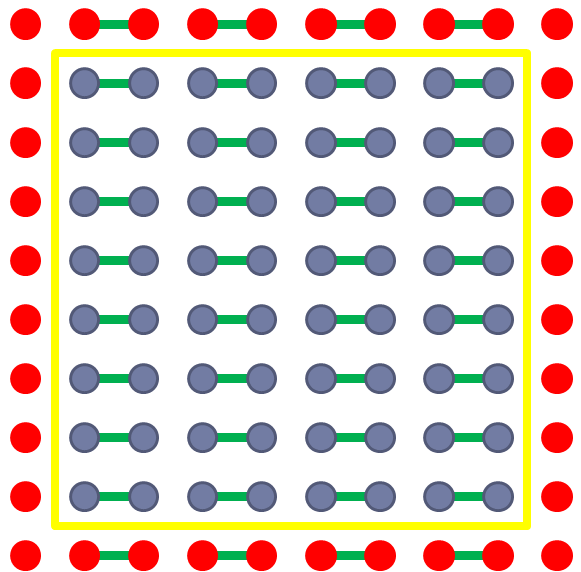
\includegraphics[width=.65\linewidth,valign=t]{my_folder/images/chunk_structural_1}
		\end{subfigure}
		\adjustbox{minipage=1.3em,valign=t}{\subcaption{}\label{fig:chunkStruct-color1}}%
		\begin{subfigure}[t]{\dimexpr.35\linewidth-1.3em\relax}
			\centering
			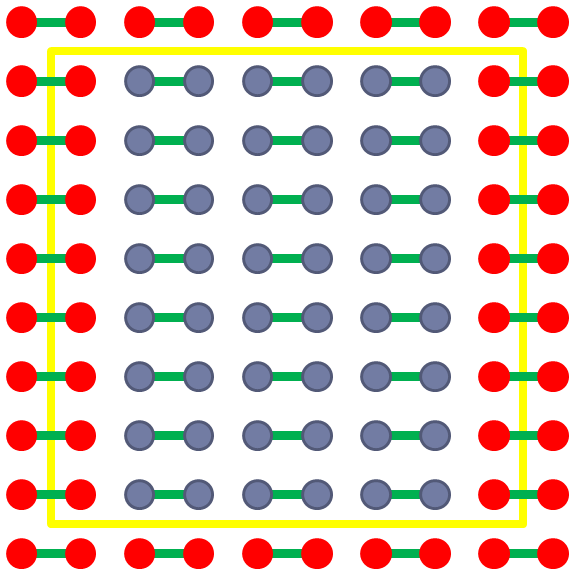
\includegraphics[width=.65\linewidth,valign=t]{my_folder/images/chunk_structural_2}
		\end{subfigure}
		\hspace*{\fill}
		\\[20pt]	
		\hspace*{\fill}
		\adjustbox{minipage=1.3em,valign=t}{\subcaption{}\label{fig:chunkStruct-color2}}%
		\begin{subfigure}[t]{\dimexpr.35\linewidth-1.3em\relax}
			\centering
			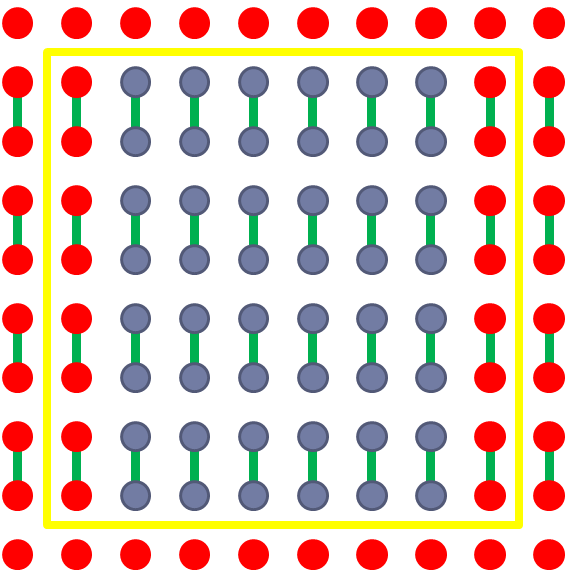
\includegraphics[width=.65\linewidth,valign=t]{my_folder/images/chunk_structural_3}
		\end{subfigure}%
		\adjustbox{minipage=1.3em,valign=t}{\subcaption{}\label{fig:chunkStruct-color3}}%
		\begin{subfigure}[t]{\dimexpr.35\linewidth-1.3em\relax}
			\centering
			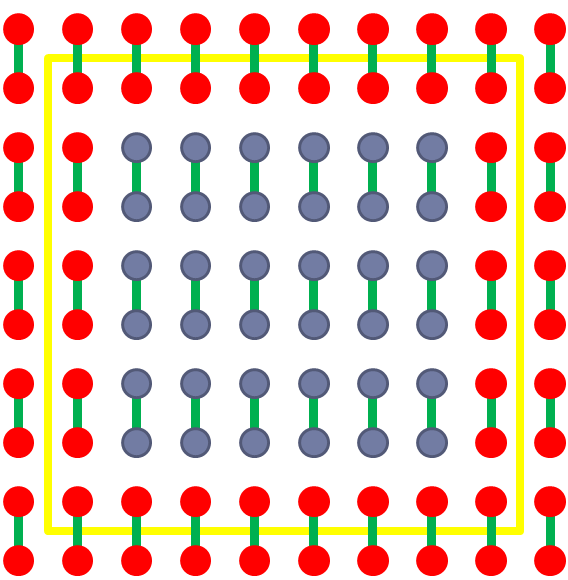
\includegraphics[width=.65\linewidth,valign=t]{my_folder/images/chunk_structural_4}
		\end{subfigure}
		\hspace*{\fill}
		\captionsetup{justification=centering} %центрировать
		\caption{Визуальная демонстрация шагов эксперимента по определению границ влияния частиц, связанных стуктурными ограничениями, при $N = 8$. Кругами обозначены вершины, зеленым обозначены обрабатываемые ребра, желтым обозначена граница подсетки $NxN$.}
		\label{fig:chunkStructExp}
	\end{figure}
	\FloatBarrier
	\newpage
	
	В результате проведения данного эксперимента, синим остаются обозначены те вершины, для вычисления положений которых достаточно только положения вершин, лежщих внутри желтой границы. Таким образом, можно разбить всю сетку ткани на пересекающиеся области (назовем их \say{заплатками}) и обсчитывать каждую \say{заплатку} в отдельной группе. При этом, подберем размер заплатки $N$ и области пересечения таким образом, чтобы частицы, соответствующие синим вершинам, полностью покрывали поверхность ткани. Тогда псевдокод шейдера для обработки структурных ограничений для \say{заплатки} будет выглядеть так, как показано на \firef{alg:structuralChunk}.
	
	\begin{algorithm} [h]
		\SetKwFunction{algoStructuralChunkPseudocode}{} 
		\SetKwProg{myalg}{Algorithm}{}{} %write in 2nd agrument <<Algorithm>>, <<Procedure>> etc
		\nonl\myalg{\algoStructuralChunkPseudocode}{
				Параллельно считать в groupshared память частицы заплатки $N$ на $N$;

				$syncPoint()$;
				
				\For{$color \in getColors(structural)$}
				{
					\ForPar{$getConstraints(structural, color)$}
					{
						$solveXPBDConstraint()$;
					}
					
					$syncPoint()$;
				}					
				
				Параллельно записать в глобальную память посчитанные частицы соответствующие синим вершинам;
		}
	\caption{Псевдокод шейдера для обработки структурных ограничений.}\label{alg:structuralChunk}
	\end{algorithm}
	
	Исходя из значений, представленных на \taref{tab:chunkSize}, было принято решение использовать $N=10$, а на каждую заплатку выделять группу из 64 потоков. Благодаря этому, достигается баланс между временем работы $GroupMemoryBarrierWithGroupSync$ и коэффициентом полезного действия (отношение синих вершин к общему числу вершин).
	
		\noindent % for correct centering
	\begin{minipage}{\textwidth}
		\vspace{\mfloatsep} % интервал 
		\centering\small
		\captionof{table}{Результаты эксперимента при разных значениях $N$ размера подсетки $NxN$}%
		\label{tab:chunkSize}
		\begin{tabular}{|c|c|c|c|}
			\hline
			\textbf{N} & \textbf{Кол-во синих} & \textbf{Кол-во красных} & \textbf{Макс. пар. ограничений}\\
			\hline
				$2$ & $0$ & $4$ & $2$\\ \hline
				$4$ & $4$ & $12$ & $8$\\ \hline
				$6$ & $16$ & $20$ & $18$\\ \hline
				$8$ & $36$ & $28$ & $32$\\ \hline
				$10$ & $64$ & $36$ & $50$\\ \hline
				$12$ & $100$ & $44$ & $72$\\ \hline
				$14$ & $144$ & $52$ & $98$\\ \hline
			
		\end{tabular}
		\vspace{\mfloatsep} % интервал 
		\normalsize %восстанавливаем шрифт 	
	\end{minipage}
	
	Данная идея обсчета ограничений заплатками может быть также применена для ограничений сдвига и ограничений изгиба и позволяет объединить в себе преимущества двух подходов представления алгоритма (\firef{alg:HeuristicParallelXPBD}). С одной стороны, количество используемых потоков неограничено, так как каждая группа будет обсчитывать свою \say{заплатку}. С другой стороны, использование $groupshared$ памяти для сохранения промежуточного результата между обработкой групп ограничений одного типа, соответствующих разным цветам рёберной раскраски, позволяет существенно уменьшить количество обращений к глобальной памяти. Помимо этого, данный подход уменьшает число переключений и вызовов шейдеров.


%% Вспомогательные команды - Additional commands
%
%\newpage % принудительное начало с новой страницы, использовать только в конце раздела
%\clearpage % осуществляется пакетом <<placeins>> в пределах секций
%\newpage\leavevmode\thispagestyle{empty}\newpage % 100 % начало новой страницы